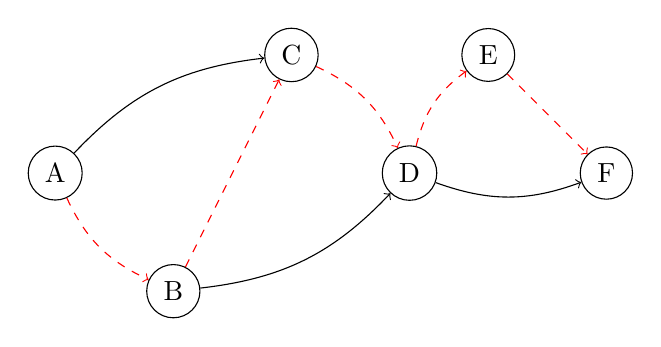
\begin{tikzpicture}
  \node[shape=circle,draw=black] (a) at (0,0) {A};
  \node[shape=circle,draw=black] (b) at (1.5,-1.5) {B};
  \node[shape=circle,draw=black] (c) at (3,1.5) {C};
  \node[shape=circle,draw=black] (d) at (4.5,0) {D};
  \node[shape=circle,draw=black] (e) at (5.5,1.5) {E};
  \node[shape=circle,draw=black] (f) at (7,0) {F};
  \path [->,red,dashed](a) edge[bend right=20] node {} (b);
  \path [->](a) edge[bend left=20] node {} (c);
  \path [->,red,dashed](b) edge node {} (c);
  \path [->,red,dashed](c) edge[bend left=20] node {} (d);
  \path [->](b) edge[bend right=20] node {} (d);
  \path [->,red,dashed](d) edge[bend left=20] node {} (e);
  \path [->,red,dashed](e) edge node {} (f);
  \path [->](d) edge[bend right=20] node {} (f);
\end{tikzpicture}
